% !TEX TS-program = xelatex
% !TEX encoding = UTF-8 Unicode
% !Mode:: "TeX:UTF-8"

\documentclass{resume}
\usepackage{zh_CN-Adobefonts_external} % Simplified Chinese Support using external fonts (./fonts/zh_CN-Adobe/)
% \usepackage{NotoSansSC_external}
\usepackage{NotoSerifCJKsc_external}
% \usepackage{zh_CN-Adobefonts_internal} % Simplified Chinese Support using system fonts
\usepackage{linespacing_fix} % disable extra space before next section
\usepackage{cite}
\usepackage{graphicx}
\usepackage{tabu}
\usepackage{multirow}
\usepackage{progressbar}

\begin{document}
\pagenumbering{gobble} % suppress displaying page number

\begin{center}
\Huge{个~~~人~~~简~~~历}
\ \\ \ 
\end{center}
\Large{
  \begin{tabu}{ c l l }
   \multirow{5}{1in}{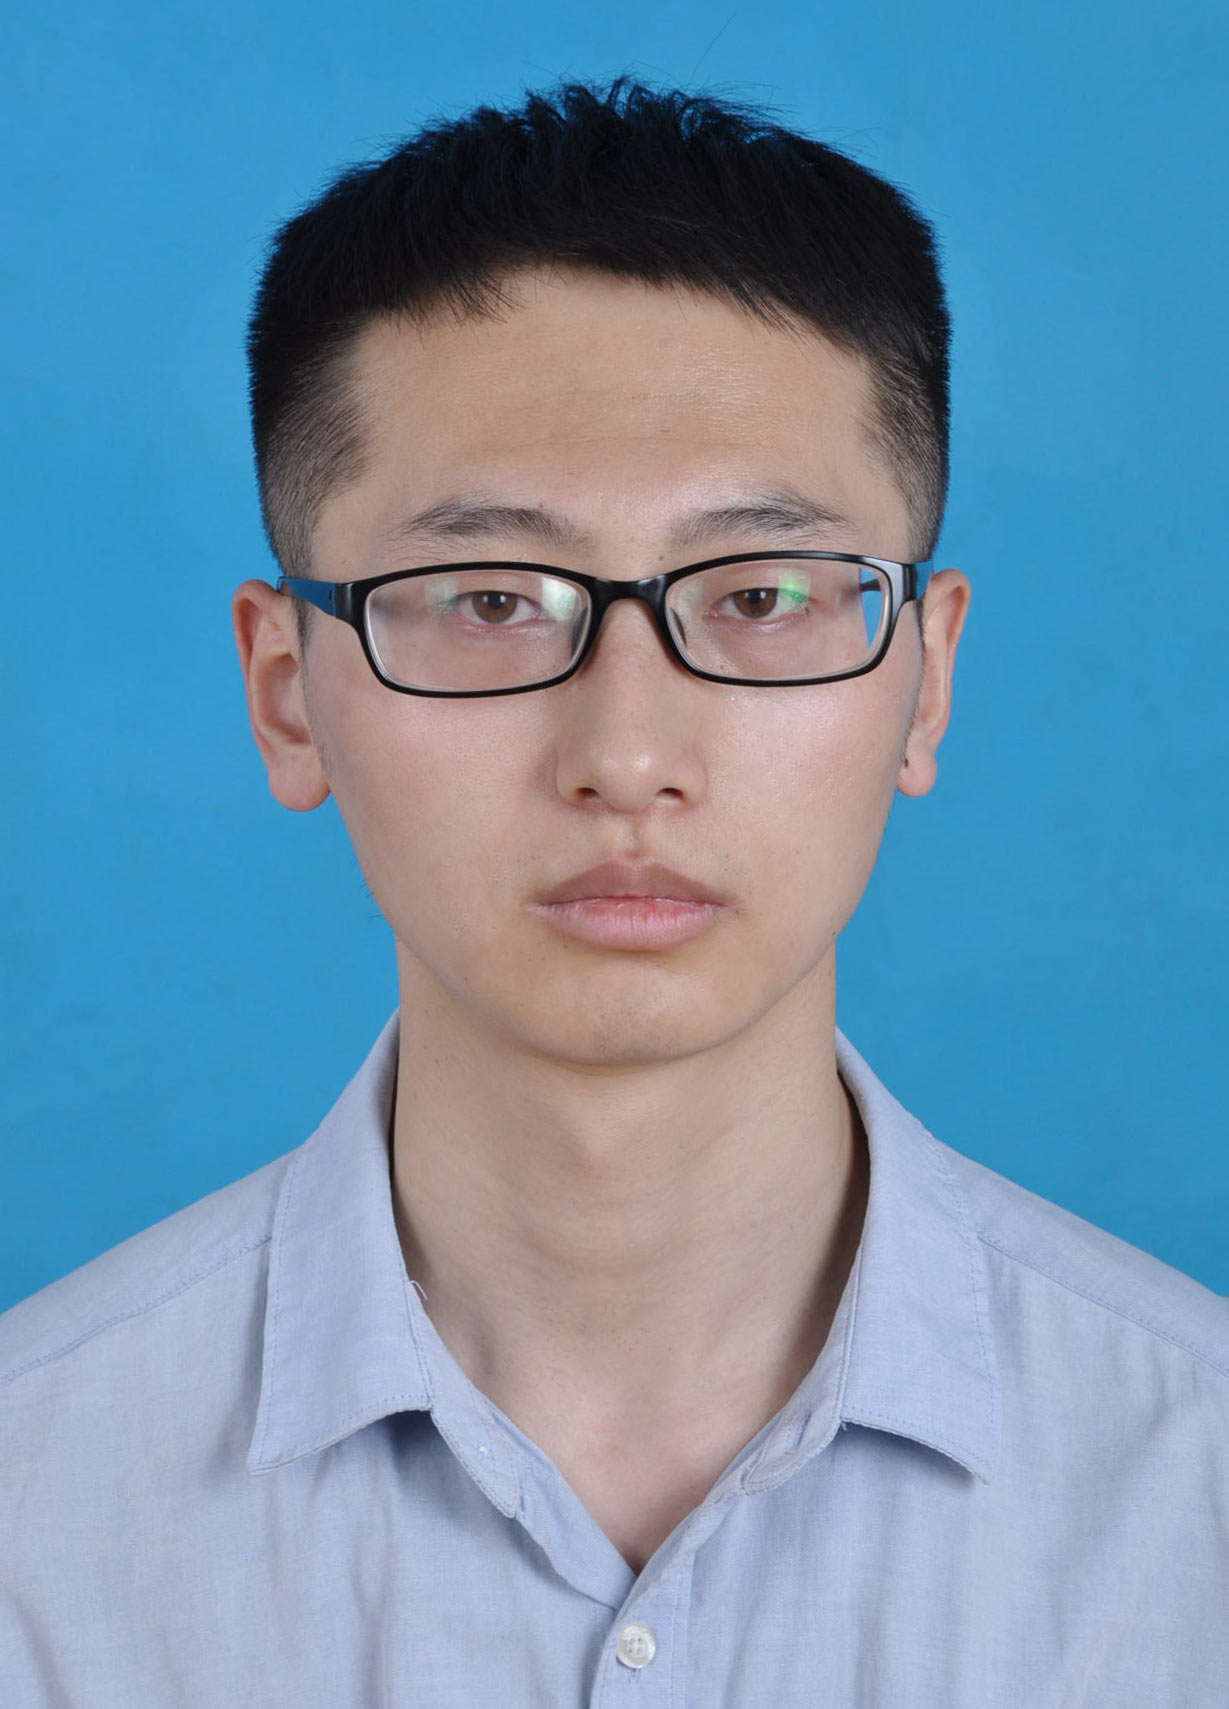
\includegraphics[width=0.88in]{avatar}} &
   \scshape{李高阳} &  \\
    & 性别:男 & 民族:汉 \\
    & 电话:(+86) 15002555080 & 生日:1995-09 \\
    & 邮箱:li.gaoyang@foxmail.com & 微信:sandbox\_ligy\\
    % & 地址:甘肃省兰州市天水南路222号 \hspace{40} & %籍贯:甘肃宁县
    & 籍贯:甘肃宁县 & 政治面貌:党员
  \end{tabu}
}

\large
\section{教育与研究经历}
\datedsubsection{\textbf{中国工程物理研究院研究生院\ 博士后}}{2023 -- 至今}
\textit{研究方向:超导异质结中的电子与自旋输运}\\
\textit{导师:唐高民\ 研究员}\\
%\textit{项目经历:自学超导理论,并在导师的指导下用非平衡格林函数结合紧束缚计算方法研究超导异质结中Andreev反射、光驱动下介观量子体系的输运现象等。}

\datedsubsection{\textbf{深圳大学\ 博士后}}{2020 -- 2023}
\textit{研究方向:金属-铁磁绝缘体异质结中的自旋输运}\\
\textit{导师:王健\ 教授}\\
%\textit{项目经历:师从王健教授学习非平衡格林函数理论与紧束缚格点数值计算方法。在导师指导下与研究组内其他博士后合作,研究金属-铁磁绝缘体异质结等体系中的量子输运现象}

\datedsubsection{\textbf{兰州大学硕博连读与中科院兰州近物所联合培养\ 博士}}{2013 -- 2019}
\textit{专业:物理学\ 理论物理\ 凝聚态理论}\\
\textit{导师:罗洪刚\ 教授(长江学者)、房铁峰\ 教授}\\
\textit{毕业论文题目:铁磁石墨烯中近藤效应的数值重整化群研究}\\
%\textit{项目经历:自学C++语言,独立编写3000行代码,在导师指导下完成数据收集与分析,完成文章撰写}

\datedsubsection{\textbf{兰州大学\ 本科}}{2009 --  2013}
\textit{专业:物理学国家基地班}

\section{发表文章}
\begin{itemize}
\item \textbf{Gao-Yang Li}, Miao-Miao Wei, Fu-Ming Xu, and Jian Wang, \textit{General method for calculating transport properties of disordered mesoscopic systems based on the nonequilibrium Green's function formalism}, Phys. Rev. B \textbf{111}, 035409 (2025).\\
研究总结:发展了一种解析计算无序体系中输运性质的理论方法。利用格林函数的Dyson方程将物理量的无序平均值展开为无序强度的级数。级数的展开系数可以用格林函数解析地给出。对多个量子体系物理量无序平均值的计算表明截断到无序的四阶已经可以在弱无序强度区域内给出准确的结果。%考虑到现有其他方法的局限性,本解析方法对无序体系中的量子输运研究具有重要意义。
\item \textbf{Gao-Yang Li} and Jian Wang, \textit{Spin transport study in disordered nonmagnetic metal/ferromagnetic insulator heterostructure based on full counting statistics within coherent potential approximation}, Phys. Rev. B \textbf{109}, 125403 (2024).\\
研究总结:发展了一种数值研究无序二维非磁金属-铁磁绝缘体异质结中自旋输运的理论方法。它基于全计数统计相干势近似(FCS-CPA),并用非平衡格林函数方法引入了平均场近似。与暴力计算的结果对比显示在弱无序情况下,两者给出相同的结果,在强无序情况下出现偏差。
\item Fu-Ming Xu, \textbf{Gao-Yang Li}, Zhi-Zhou Yu, Lei Zhang, Bai-Geng Wang, and Jian Wang, \textit{Unified framework of the microscopic Landau-Lifshitz-Gilbert equation and its application to skyrmion dynamics}, Phys. Rev. B \textbf{108}, 144409 (2023). 共同一作。\\
研究总结:基于非平衡格林函数方法,推导了描述磁矩动力学特性的Landau- Lifshitz-Gilbert equation (LLG方程)的微观理论。利用这一理论,数值研究了磁性斯格明子的量子参数泵浦特性,揭示了斯格明子在外加周期性驱动势场下在空间中的运动等动力学特征。
\item \textbf{Gao-Yang Li}, Fu-Ming Xu, and Jian Wang, \textit{Universal behavior of magnon-mediated spin transport in disordered NM/NM/FI heterostructure}, Front. Phys. \textbf{18}, 33310 (2023).\\
研究总结:系统研究了在Anderson无序下,非磁金属-铁磁绝缘体异质结中由磁振子辅助的自旋输运的统计行为,发现在二维情况下,弱无序会增强自旋流的输运,这与传统的正常金属中无序总是抑制输运的结果相背。在二维体系的弱无序区,作者发现了一个新的标度关系,即自旋电导的涨落与其均值成正比,且此标度关系是普适的。
\item \textbf{Gao-Yang Li}, Hao-Jin, Ya-Dong Wei, and Jian Wang, \textit{Giant effective electron-magnon coupling in a nonmagnetic metal–ferromagnetic insulator heterostructure}, Phys. Rev. B \textbf{106}, 205303 (2022).\\
研究总结:基于非平衡格林函数方法发展了计算非磁性金属/铁磁绝缘体异质结中自旋电导的量子自旋输运的理论。文章考虑了界面处的sd相互作用,得到了自洽玻恩近似下自旋流的表达公式。并将它用于模拟实验材料构型,定性解释了实验结果,并提供了实验上得到更大自旋电导的可行指导。
\item Wan-Xiu He, Zhan Cao, \textbf{Gao-Yang Li}, Lin Li, Hai-Feng Lü, ZhenHua Li, and Hong-Gang Lo, \textit{Performance of the T-matrix based master equation for Coulomb drag in double quantum dots}, Phys. Rev. B \textbf{101}, 035417 (2020).\\
研究总结:基于级联运动方程方法,研究了双量子点体系中的库仑拖拽效应。评估了基于T-矩阵的主方程方法(TME)在研究弱耦合区域库仑拖曳中的准确性。尽管 TME 能够捕捉部分定性趋势,但在存在较大电荷波动和四阶隧穿过程的系统中,其定量预测表现不佳。研究明确了 TME 的可靠应用范围,为库仑拖拽的进一步研究提供了指导。
\item \textbf{Gao-Yang Li}, Tie-Feng Fang, Ai-Min Guo, and Qing-Feng Sun, \textit{Ferromagnetism-induced Kondo effect in graphene with a magnetic impurity}, Phys. Rev. B \textbf{100}, 115115 (2019).\\
研究总结:使用数值重整化群方法研究了铁磁性石墨烯中的磁性吸附原子产生的Kondo效应。研究表明,铁磁性不仅不会削弱 Kondo关联,还会随着狄拉克电子自旋极化的增强提高Kondo温度。此外,在掺杂石墨烯中,发现了只出现在特定自旋方向上的异常 Kondo 共振。这一发现拓展了对铁磁性材料中 Kondo 物理的理解。
\end{itemize}

% \section{未来研究兴趣}
% \begin{itemize}%[parsep=0.5ex]
% \item 磁振子系统的交流驱动
% \item 铁电体系的电子输运
% \end{itemize}

\section{自我评价}
\qquad 自认为是一个上进努力有责任心的人,能和周围的人和睦相处,进行高效的交流。自学能力强,对新知识有较高的学习热情,能够自驱地学习需要的知识,并能投入精力解决问题。

\section{兴趣爱好}
\qquad 羽毛球

% \section{个人主页}
% \rm{https://github.com/GoldenRaven}

%% Reference
% \newpage
% \bibliographystyle{IEEETran} \bibliography{mycite}
\end{document}
